\chapter{Architecture}

\begin{figure}
	\centering
	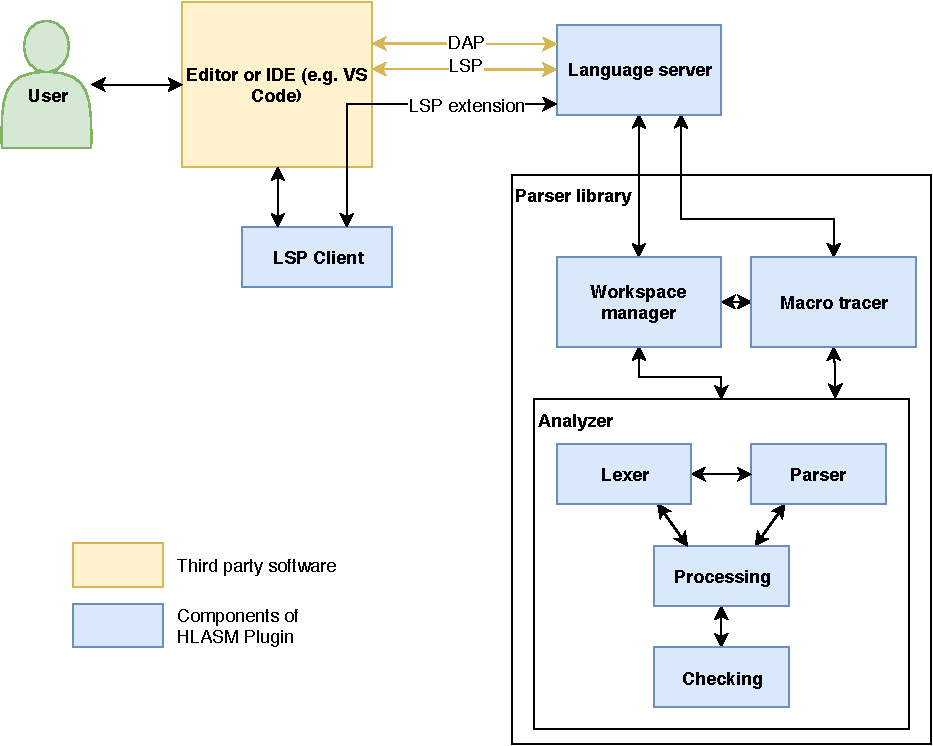
\includegraphics[width=\textwidth]{img/hlasm_architecture}
	\caption{The architecture of HLASM Plugin}
	\label{fig03:arch}
\end{figure}

 The architecture is based on the way modern code editors and IDEs are extended to support additional languages. We chose to implement Language Server Protocol \footnote{https://microsoft.github.io/language-server-protocol/} (LSP), which is supported by majority of contemporary editors.

In LSP the two parties who communicate are called \emph{client}  and \emph{language server}. The client runs as an extension of development tool. All language-specific user actions are transformed into standard LSP messages and sent to the language server, which analyses the source code and sends back response, which is then interpreted and presented to the user in editor-specific way. This architecture makes possible to have only one LSP client implementation for each code editor which may be reused by all programming languages. And vice versa, every language server may be easily used by any editor that has an implementation of LSP client.

To add support for HLASM we have to implement LSP language server and write thin extension to an editor, which will use already existing implementation of LSP client. 

This chapter presents decomposition of the project into smaller components and describes their relations. The overall architecture is pictured in Figure~\ref{fig03:arch}.

\section{Language server}

The responsibility of the Language server component is to implement the LSP and pass all the  The issues that it addresses:

\begin{itemize}
    \item To read LSP messages from standard input or TCP and write responses.
    \item To parse JSON RPC to C++ structures so they can be further used.
    \item To serialize C++ structures into JSON, so it can be sent back to client.
    \item Implement asynchronous request handling. For example when user makes several consecutive changes to a source code, it is not needed to parse every change, only the final version.
\end{itemize}

\section{Parser library}

Parser library is the core of the project --- it encapsulates all parsing capabilities. It keeps track of opened files in the editor and provides information about them. It has API based on LSP --- every relevant request and notification has corresponding method in parsing library. The API includes:

\begin{itemize}
	\item Implementation of text synchronization notifications (didOpen, didChange, didClose), which inform the library about files that are currently opened in the editor and their exact contents.
	\item Implementation of workspace management notifications (DidChangeWorkspaceFolders): many editors have possibilities to open more workspaces in the same time, the parser library supports this too. Workspace is basically just a folder which contains related source codes. Workspaces help parser library find macro and copy files.
	\item A method to consume DidChangeWatchedFiles notification which makes it possible to react to workspace changes that were not made by the user in editor, but still may affect the parsing. For example when user deletes an external macro file, the parser library should react by reporting that it cannot find the macro.
	\item Implementation of diagnostics publishing (publishDiagnostics notification). A diagnostic is used to indicate a problem with source files, such as compiler error or warning. The parser library provides a callback to let language server know that diagnostics have changed.
	\item Callback for highlighting information provision.
	\item Implementation of language feature requests (definition, references, hover, completion), which provide information needed for proper reaction of the editor on user actions.
	
\end{itemize}

The parser library is further decomposed into smaller components.

\subsection{Analyser}

Analyser is able to process a single HLASM file. The processing includes:
\begin{itemize}
 \item Recognition of statements and their parts (lexing and parsing).
 \item Interpretation of instructions that should be executed in compile time.
 \item Check whether the HLASM source code is well-formed.
 \item Report problems with the source by producing LSP diagnostics.
 \item Provide highlighting and LSP information.
\end{itemize}


\subsubsection{Lexer}
\subsubsection{Parser}
\subsubsection{Processing}
\subsubsection{Checking}


\subsection{Workspace manager}









\subsection{Macro tracer}



\section{VS code client}

mirko:

a je fajn rozepsat vsechny API a takovy veci co sou po ceste

--velky graf vsetkych komponent
--ku kazdemu odstavcek 